\documentclass{ws-procs11x85}
\usepackage{ws-procs-thm}
\usepackage{graphicx}

\begin{document}

\title{Held-Out Cell Lines Are Not Held-Out Combinations:\\
Auditing Evaluation Protocols for Drug Combination Synergy Prediction}

\author{Kusal Debnath and Preetam Ghosh$^\dag$}

\address{Department of Computer Science, Virginia Commonwealth University,\\
Richmond, Virginia 23284, USA\\
$^\dag$E-mail: pghosh@vcu.edu}

\begin{abstract}
Computational prediction of drug-combination synergy is evaluated on benchmarks
derived from combinatorial screens, in which a fixed panel of drug pairs is
assayed across a fixed panel of cell lines. Recognising that uniformly random
splits over measurements are permissive, the field has adopted cold-start
protocols --- leave-drug-out, leave-cell-line-out, leave-tissue-out. We show that
holding out a cell line does not hold out a combination. Within a single screen
the result is exact and follows from the screen's own design: because a screen
assays its pair matrix across its entire cell panel, leave-cell-line-out retains
100\% of test combinations in training, on each of the four contributing screens
we examine. Pooled over a harmonised DrugComb corpus of 180,746 feature-complete
measurements the figure is 72.8\%, pooling diluting the effect rather than
reducing it. We quantify the consequence with a null model using no molecular
information --- a per-cell-line mean plus a per-pair mean. Under
leave-cell-line-out this null model significantly outperforms both a symmetric
neural baseline ($+0.055$ Pearson, $p = 0.0006$) and a 4.5M-parameter
pathway-aware model ($+0.122$, $p = 0.0003$), while collapsing to 0.200 when
combinations are held out. Using the pathway model as an instrument, we find that
the sign of a small structure effect flips with protocol: structure helps where
combinations are held out ($+0.025$, $p < 0.0001$) and hurts where cell lines are
($-0.067$, $p = 0.0018$), with two further protocols showing no resolvable
difference. Component ablation attributes far more of the model's advantage to
imputation of missing drug--target annotations ($-0.158$ when removed) than to
pathway topology ($-0.017$). The distinction that matters is between predicting a
known combination in an uncharacterised context --- legitimate and clinically
relevant --- and combination generalisation; one number cannot serve both. We
release the audit, the null model, and fingerprinted split definitions so overlap
can be reported alongside any cold-start result at negligible cost.
\end{abstract}

\keywords{Drug combination synergy; evaluation methodology; data leakage;
benchmark design; null models.}

% required, do-not-remove
\copyrightinfo{\copyright\ 2026 The Authors. Open Access chapter published by World Scientific Publishing Company and distributed under the terms of the Creative Commons Attribution Non-Commercial (CC BY-NC) 4.0 License.}

\section{Introduction}\label{sec:intro}

Combination therapy is standard in oncology, and the candidate space is far too
large to screen exhaustively: for $n$ compounds across $m$ cell lines it grows as
$O(n^2m)$. Computational prioritisation is therefore attractive, and a
substantial literature has developed since DeepSynergy first applied deep
learning to the problem.\cite{preuer2018} Reviews count more than thirty
machine-learning methods published since 2021 alone.\cite{abbasi2024,pan2023}

Progress is measured against benchmarks derived from combinatorial screens ---
O'Neil,\cite{oneil2016} NCI-ALMANAC,\cite{holbeck2017} and their aggregation in
DrugComb.\cite{zagidullin2019,zheng2021} These screens share a design property
that is a virtue experimentally and a hazard statistically: a fixed panel of drug
pairs is assayed across a fixed panel of cell lines. The resulting data is dense
in \emph{contexts per combination} and sparse in \emph{distinct combinations}.

The field knows random splits are permissive here. Preuer et al.\ evaluated on
novel combinations rather than random measurements as early as 2018, and reported
that every method they compared degraded when extrapolating to unexplored drugs
or cell lines.\cite{preuer2018} Dewulf et al.\ formalised the cold-start subtasks
for drug--drug interaction prediction and argued that matched validation schemes
are critical to correct assessment.\cite{dewulf2021} Contemporary methods
routinely report leave-drug-out, leave-combination-out and leave-cell-line-out
alongside headline numbers.\cite{monem2024,boonyarit2025,alam2024}

This is a specific instance of a general problem. Kapoor and Narayanan surveyed
seventeen scientific fields and found leakage affecting 294 papers, sometimes
producing wildly overoptimistic conclusions; in their reproducibility study of
civil-war prediction, correcting leakage removed the entire advantage of complex
models over decades-old logistic regression.\cite{kapoor2023,kapoor2022} Bernett
et al.\ note that leakage is especially hard to detect in biological data because
of complex dependencies between samples,\cite{bernett2024} and Rosenblatt et al.\
show that repeated subjects drastically inflate performance in connectome
models\cite{rosenblatt2024} --- the direct structural analogue of repeated drug
pairs.

We ask a question that, to our knowledge, has not been measured: \textbf{within
each cold-start protocol, how much combination overlap actually survives?}
Holding out a cell line removes a \emph{context}; it does not remove a
\emph{combination}, because the same pair is measured in the cell lines that
remain. Whether that matters is an empirical question about how redundant the
screens are.

\paragraph{Contributions.}
(1) \textbf{A protocol audit} (Sec.~\ref{sec:overlap}). Across six protocols we
measure the fraction of test combinations also present in training.
Leave-cell-line-out retains 72.8\% and leave-tissue-out 56.4\%; within a single
screen, leave-cell-line-out retains 100\% by construction.
(2) \textbf{A null model quantifying the consequence} (Sec.~\ref{sec:invert}). A
per-cell plus per-pair mean, using no molecular information, significantly
outperforms two neural models under leave-cell-line-out. We argue it should be
reported routinely.
(3) \textbf{A demonstration that the protocol determines the verdict}
(Sec.~\ref{sec:verdict}). On one architecture and corpus, the \emph{sign} of a
small structure effect flips with the protocol --- positive where combinations
are held out, negative where cell lines are, with two protocols showing no
resolvable difference.
(4) \textbf{A component attribution} (Sec.~\ref{sec:ablation}). The pathway model
relies far more on imputing missing drug--target annotations ($-0.158$ Pearson
when removed) than on pathway topology ($-0.017$), suggesting benefits attributed
to biological priors may partly reflect database completion.

We are explicit about what we do \emph{not} claim. We do not claim published
results are invalid: we read the methods sections of three widely-cited methods
and found their protocols sound (Sec.~\ref{sec:verified}). We do not claim
pathway representations are unhelpful in general; we test one architecture. The
claim concerns what a class of protocols measures, and holds regardless of how
carefully any individual paper was executed.

\section{Background and Related Work}

\subsection{Synergy quantification}

Synergy is defined relative to a reference model of non-interaction, and the
common references --- Loewe additivity, Bliss independence, highest single agent,
zero interaction potency --- rest on different assumptions and disagree in
practice.\cite{vlot2019,duarte2022,roell2017} Vlot et al.\ found multiple
instances of strong disagreement between the four on the Merck screen despite
moderate overall concordance,\cite{vlot2019} and the choice of dose--response
fitting software can flip a combination between synergistic and
antagonistic.\cite{fuentealba2023} Implementations are available in
SynergyFinder.\cite{ianevski2022} We use Loewe throughout and note in
Sec.~\ref{sec:limits} that our overlap measurement is metric-independent while
our performance results are not.

\subsection{Cold-start protocols}

Dewulf et al.\ identify the distinct subtasks arising when drugs, pairs or
contexts are novel, and propose matched validation schemes.\cite{dewulf2021} Our
protocols follow this taxonomy; our contribution is measuring residual overlap
\emph{within} each scheme rather than proposing the schemes. Yousefabadi et al.\
state that permissive cross-validation allowing drug pairs across folds inflates
performance, and adopt pair-held-out validation for antibacterial
synergy.\cite{yousefabadi2025} Abbasi and Rousu's review concludes methods
perform well for known drugs and cell lines but fall short for novel
ones.\cite{abbasi2024} Agboola et al.\ report a random forest outperforming their
deep model under cold-drug validation and interpret it
transparently\cite{agboola2026} --- a precedent for the null-model result we
report.

\subsection{We verified, and do not allege, protocol failures}\label{sec:verified}

Reading methods sections rather than abstracts: DeepSynergy's headline 0.73
Pearson is for ``novel drug combinations within the space of explored drugs and
cell lines'' --- combination hold-out.\cite{preuer2018} Monem et al.\ state their
five-fold split ensures ``each drug-drug combination is included in only
one-fold''.\cite{monem2024} SynProtX partitions randomly 80:20 for its headline
and reports cold-start scenarios separately.\cite{boonyarit2025} Reported gains
over DeepSynergy are, on this evidence, protocol-matched. The problem we identify
is not that these papers erred; it is that a protocol they all use measures less
than its name implies.

\subsection{Structure-informed synergy models}

Incorporating pathway or network structure is an active direction:
network-proximity approaches,\cite{cheng2019} pathway-activation
scores,\cite{trac2025} interpretable subsystem models,\cite{kuenzi2020} graph and
transformer architectures,\cite{alam2024,kuru2022,sherine2025} multi-task
formulations,\cite{chen2023,wang2023} multi-omics
ensembles,\cite{preto2022,lin2023} and proteomics-based
models.\cite{boonyarit2025} Our instrument model belongs to this family; we use
it to ask what such a model relies on, not to advance the family.

\subsection{Leakage in ML-based science}

Our finding instantiates a documented failure mode. Kapoor and Narayanan's
taxonomy of eight leakage types includes non-independence between train and test
samples;\cite{kapoor2023,kapoor2022} REFORMS provides a reporting
checklist;\cite{kapoor2024} Bernett et al.\ give biology-specific guiding
questions;\cite{bernett2024} Rosenblatt et al.\ quantify the effect in
neuroimaging;\cite{rosenblatt2024} and reviews in other applied fields document
the same pattern.\cite{zhu2023,semmelrock2024} What is distinctive here is that
the subfield already adopted a remedy --- cold-start protocols --- and the remedy
is incomplete in a way that is invisible without counting pairs.

\section{Methods}

\subsection{Corpus}

We harmonise DrugComb\cite{zagidullin2019} to 634,631 measurements after removing
self-pairs and rows lacking a Loewe score: 73,108 unique unordered pairs across
288 cell lines, a mean of 8.68 cell lines per pair (max 127). Requiring complete
drug and cell features leaves 180,746 measurements over 1,945 drugs, 159 cell
lines and 15 tissues, drawn principally from ALMANAC, FRIEDMAN, ONEIL and
ASTRAZENECA.

Every protocol, split, overlap figure and performance number reported below is
computed on this feature-complete subset of 180,746 measurements, not on the full
634,631; we state this explicitly because the distinction is precisely the kind
this paper argues should be made. The filter preferentially retains
well-characterised drugs, which appear in more pairs, so it plausibly biases the
pooled overlap \emph{upward}. Two things limit the concern: the per-screen
replication in Sec.~\ref{sec:overlap} reaches 100\% by construction and so cannot
be inflated by it, and {\tt leave\_combo\_out} and {\tt leave\_drug\_out} reach
0\% regardless. We use the DrugComb v1.5 release\cite{zheng2021}.

\subsection{Protocols}

Six protocols are implemented over the common corpus, each persisted as row
indices with a corpus fingerprint so a split replays exactly without
redistributing data: {\tt random}, {\tt leave\_combo\_out} (unseen combination,
both drugs seen), {\tt leave\_drug\_out} ({\tt one}/{\tt both} variants), {\tt
leave\_cell\_out}, {\tt leave\_tissue\_out}, {\tt leave\_study\_out}.

Grouped protocols assign entities by mass-aware greedy packing rather than
uniform partitioning. The drug degree distribution is heavy-tailed and naive
partitioning is unstable --- an early implementation produced 297,039 test rows
against 11,935 training rows. The packer orders groups by row mass, assigns each
to the bin with the largest remaining deficit, and asserts the achieved test
fraction lies in $[0.05, 0.25]$ before a split is accepted.

That assertion applies to the mass-packed protocols only. {\tt
leave\_tissue\_out} and {\tt leave\_study\_out} partition on an explicit
categorical assignment, so their test fraction is whatever the held-out block
happens to weigh and the check is deliberately waived; we note this because a
single held-out tissue can exceed the band substantially. {\tt
leave\_tissue\_out} is restricted to the eight tissues with at least 3,500
covered rows, the distribution being severely skewed (skin 31.4\% of covered
rows; pancreas 6 rows). Prostate, listed as eligible in an earlier version of our
code, in fact holds 3,293 rows and is excluded.

\paragraph{Overlap metric.} For a split we report the fraction of test unordered
pairs that also appear in training. This requires no model and no training; it is
a property of the partition, computable in seconds.

\subsection{Baselines}

\textbf{B1}, the null model, predicts a per-cell-line mean plus a per-pair mean
deviation, both estimated on training rows only, backing off to the global mean
for unseen entities. It uses no structure, targets, pathways or omics. Its role
is diagnostic: a benchmark on which B1 is competitive is one whose signal is
largely recoverable from which pair and which context, without chemistry.

We also report \textbf{B2}, gradient boosting on PCA-reduced embeddings --- a
learned but non-neural comparator that sits between B1 and the neural models ---
and \textbf{B3}, a symmetric MLP over drug embeddings and cell features with no
ontology, graph or target projection, the reference for ``does structure help''.

\subsection{The instrument model}

Pathway vocabulary, gene membership, graph topology and mechanism taxonomy are a
versioned specification rather than code, so no assumption about relevant biology
is embedded in the architecture. We use MSigDB Hallmark (50 gene
sets)\cite{liberzon2015} and aggregate a pathway--pathway graph from STRING v12
physical interactions at combined score at least 700\cite{szklarczyk2023} with no
hand-specified edges; panel genes absent from every Hallmark set --- much of the
druggable kinome, since Hallmark sets are expression-response signatures --- are
placed by STRING guilt-by-association (19 of 20 automatically). Drug target
profiles project onto pathways, compose across the pair over the graph, and read
out through a synergy head. 4.5M parameters.

Cell context is 160 dimensions: 14 PROGENy activities,\cite{schubert2018} 64
principal components of protein-coding expression, 64 of CRISPR gene effect over
the ontology's gene universe, and 18 genotype flags, all from the DepMap
portal\cite{tsherniak2017} ({\tt CRISPRGeneEffect.csv}, {\tt
OmicsExpressionTPMLogp1HumanProteinCodingGenes.csv} and {\tt
OmicsSomaticMutations.csv}; 18,531 genes across 1,208 cell lines). Drug structure
uses MolFormer embeddings.\cite{ross2022} Drug--target profiles come from ChEMBL\cite{zdrazil2024}
over a 72-gene panel; only 24.7\% of trainable rows have both drugs annotated, so
a target-imputation head predicts profiles from structure (5-fold leave-drug-out
macro-AUPRC 0.219, versus 0.162 nearest-neighbour and 0.064 prevalence prior).

\subsection{Statistics and reproducibility}\label{sec:stats}

Comparisons use 6 seeds (1--5, 42) for {\tt random}, {\tt leave\_combo\_out},
{\tt leave\_drug\_out} and {\tt leave\_cell\_out}, where each seed redraws
\emph{both} the split partition and the model initialisation, since which pairs
land in test is itself a large source of spread.

\textbf{{\tt leave\_tissue\_out} and {\tt leave\_study\_out} are deterministic by
construction:} their partitions are fixed by an explicit tissue or study
assignment, so the three seeds we run vary only the model initialisation and the
split is identical across them. Their variances are therefore not comparable to
the other four protocols' and are systematically smaller --- a paired standard
deviation of 0.001 in Sec.~\ref{sec:invert} reflects a fixed partition, not an
unusually stable estimate. We report them as single-partition results with
$n = 3$ initialisations and exclude them from the abstract's headline claims. Model-versus-model comparisons are paired on the shared
split and tested with a paired $t$-test. Targets are winsorised at the 0.5\%
quantile fitted on training rows only, then standardised; errors are reported in
raw Loewe units.

\paragraph{Resolution floor.} Repeating an identical configuration --- same seed,
same split, same code path --- reproduces to within 0.007 Pearson, reflecting
non-deterministic GPU kernels. We therefore treat unpaired differences below
about 0.01 as unresolved and say so where relevant (Sec.~\ref{sec:ablation}).
Paired differences are considerably tighter, because both models absorb the same
run-level noise.

\section{Results}

\subsection{Combination overlap survives cold-start protocols}\label{sec:overlap}

Table~\ref{tab:overlap} reports the fraction of test combinations also present in
training. The result is specific rather than a blanket dismissal. {\tt
leave\_study\_out} retains only 9.8\%, because separate screens use largely
disjoint drug panels: partitioning by \emph{data source} approximates combination
novelty, while partitioning by \emph{biological context} does not.

\begin{table}[ht]
\tbl{Fraction of test combinations also present in training, on the partitions
all reported results use. Mean $\pm$ s.d.\ over 6 seeds, except the two
deterministic protocols (Sec.~\ref{sec:stats}), which have a single partition.
See Fig.~\ref{fig:overlap}A.}
{\begin{tabular}{@{}lrrl@{}} \toprule
protocol & test rows & test pairs also in train & holds out combinations \\ \colrule
{\tt random} & 18,076 & 94.0\% $\pm$ 0.3\% & no \\
{\tt leave\_cell\_out} & 18,076 & \textbf{72.8\% $\pm$ 0.1\%} & \textbf{no} \\
{\tt leave\_tissue\_out} & 71,638 & \textbf{56.4\%} (fixed) & \textbf{no} \\
{\tt leave\_study\_out} & 15,279 & 9.8\% (fixed) & mostly \\
{\tt leave\_drug\_out} & 31,728 & 0.0\% & yes \\
{\tt leave\_combo\_out} & 18,074 & 0.0\% & yes \\ \botrule
\end{tabular}}
\label{tab:overlap}
\end{table}

\paragraph{Within a single screen the overlap is total.} Each contributing study
is an independent screen with its own panels and protocol; repeating the audit
inside each is a stronger test than the pooled corpus (Table~\ref{tab:perstudy},
Fig.~\ref{fig:perstudy}). The pooled figure of 72.8\% \emph{understates} the
problem --- pooling dilutes overlap by mixing in pairs unique to other screens.
On O'Neil, the benchmark DeepSynergy introduced and still the field's most
common, a predictor with no molecular information reaches 0.682 under a random
split and 0.600 under leave-cell-line-out.

\begin{table}[ht]
\tbl{Per-study replication. Overlap with B1 Pearson in parentheses.}
{\begin{tabular}{@{}lrrrlll@{}} \toprule
study & rows & pairs & rows/pair & {\tt random} & {\tt leave\_cell\_out} & {\tt leave\_combo\_out} \\ \colrule
ALMANAC & 109,897 & 2,992 & 36.7 & 100\% (0.677) & 100\% (0.653) & 0\% (0.057) \\
FRIEDMAN & 50,107 & 2,926 & 17.1 & 100\% (0.380) & 100\% (0.400) & 0\% (0.100) \\
ONEIL & 9,369 & 315 & 29.7 & 100\% (0.682) & 100\% (0.600) & 0\% (0.135) \\
ASTRAZENECA & 5,910 & 407 & 14.5 & 100\% (0.421) & 92\% (0.298) & 0\% (0.323) \\ \botrule
\end{tabular}}
\label{tab:perstudy}
\end{table}

\subsection{The overlap is large enough to invert model rankings}\label{sec:invert}

Protocols in Table~\ref{tab:main} are ordered by overlap, and B1 broadly tracks
it ($r = 0.96$, $p = 0.003$; Spearman $\rho = 0.81$, $p = 0.05$). We deliberately
do not lean on this. It is a correlation over six protocols, not six independent
observations of a mechanism, and it does not survive scrutiny as a causal
statement: at essentially zero overlap B1 still ranges from 0.111 ({\tt
leave\_study\_out}) to 0.200 ({\tt leave\_combo\_out}), a spread of 0.089 that
exceeds the $+0.055$ leave-cell-line-out gap the ordering is meant to explain.
Something besides combination overlap moves B1 by more than the effect in
question. The load-bearing evidence in this paper is the per-screen 100\% result
of Sec.~\ref{sec:overlap}, which is exact and needs no model; the correlation is
a supporting observation only.

\begin{table}[ht]
\tbl{Pearson correlation on Loewe. Mean over 6 seeds (3 initialisations for the
two deterministic protocols). B2 is gradient boosting on PCA-reduced embeddings.
See Fig.~\ref{fig:overlap}B.}
{\begin{tabular}{@{}lrrrrr@{}} \toprule
protocol & overlap & B1 (no chemistry) & B2 (GBM) & B3 (MLP) & pathway model \\ \colrule
{\tt random} & 94.0\% & 0.588 & 0.630 & 0.745 & 0.744 \\
{\tt leave\_cell\_out} & 72.8\% & \textbf{0.425} & 0.375 & 0.370 & 0.304 \\
{\tt leave\_tissue\_out} & 56.4\% & \textbf{0.325} & 0.277 & 0.202 & 0.211 \\
{\tt leave\_study\_out} & 9.8\% & 0.111 & 0.146 & 0.139 & 0.123 \\
{\tt leave\_drug\_out} & 0.0\% & 0.125 & 0.216 & 0.245 & 0.224 \\
{\tt leave\_combo\_out} & 0.0\% & 0.200 & 0.378 & 0.594 & \textbf{0.618} \\ \botrule
\end{tabular}}
\label{tab:main}
\end{table}

Under {\tt random}, B1 recovers 79\% of a neural model's correlation using no
molecular information. Its drop once combinations are held out is $0.388 \pm
0.008$ --- a tight estimate of what the protocol, rather than the model, was
contributing.

\textbf{B1 beats both neural models on both high-overlap cold-start protocols},
paired over seeds. Under leave-cell-line-out: B1 $-$ MLP $= +0.055$ ($t = 7.71$,
$\mathrm{df} = 5$, $p = 0.0006$) and B1 $-$ pathway model $= +0.122$ ($t = 8.81$,
$\mathrm{df} = 5$, $p = 0.0003$). Under leave-tissue-out, on a single fixed
partition with three initialisations: B1 $-$ MLP $= +0.123$ ($t = 11.85$,
$\mathrm{df} = 2$, $p = 0.007$) and B1 $-$ pathway model $= +0.113$ ($t = 158.2$,
$\mathrm{df} = 2$, $p = 0.00004$). The very large $t$ in the last comparison is
an artefact of the fixed partition, not evidence of a stronger effect: B1 is a
deterministic function of the split and so is constant across the three runs,
leaving only the pathway model's initialisation variance (paired s.d.\ 0.001) in
the denominator. We report it for completeness and rest the claim on the
leave-cell-line-out arm, where the partition is redrawn.

The result is not peculiar to one hand-built null model. B2, an off-the-shelf
gradient-boosting regressor, also exceeds both neural models under high overlap
(Table~\ref{tab:main}) while losing to them by a wide margin ($0.378$ vs $0.594$)
once combinations are held out. We state the margins precisely rather than lean
on the direction: under leave-cell-line-out B2 beats the pathway model
comfortably ($+0.071$) but only matches the MLP ($+0.005$, inside the 0.007
resolution floor of Sec.~\ref{sec:stats}). B2 is also a different function class,
not the controlled comparison --- an MLP handed the identifiable two-way
structure --- that would settle the question; we name that experiment in
Sec.~\ref{sec:limits}. What B2 does establish is that the effect is not an
artefact of one tailored null model.

Eight paired tests are reported in this paper without correction for multiple
comparisons. At a Bonferroni threshold of $\alpha = 0.05/8 = 0.00625$ all
comparisons we describe as significant clear it except the leave-tissue-out
B1 $-$ MLP result ($p = 0.007$), which sits just outside and should be read as
borderline.

Conversely, {\tt leave\_study\_out} --- the only protocol besides combination
hold-out with low overlap --- is hard for everything: B1 reaches 0.111 and the
pathway model 0.123, both near the floor. A protocol that genuinely removes
combination overlap produces uniformly low numbers, which is what a hard task
should look like. This mirrors Kapoor and Narayanan's civil-war result, where
correcting leakage removed the advantage of complex models over logistic
regression.\cite{kapoor2023}

\begin{figure}[ht]
\centerline{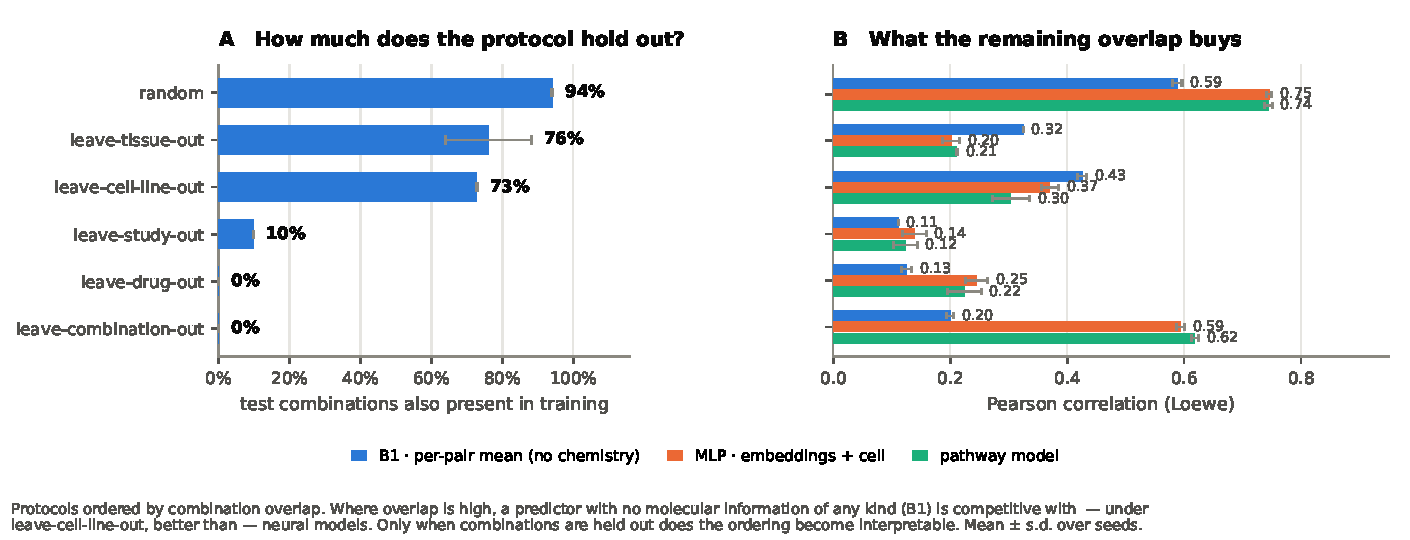
\includegraphics[width=\textwidth]{fig1_overlap_vs_nullmodel.pdf}}
\caption{(A) Combination overlap by protocol. (B) What that overlap buys each
method. Protocols are ordered by overlap; the null model B1 tracks it at $r =
0.92$.}
\label{fig:overlap}
\end{figure}

\subsection{The protocol determines the verdict}\label{sec:verdict}

Table~\ref{tab:verdict} contains one small positive effect, one small negative
effect, and two null results. We resist the temptation to call this ``three
incompatible conclusions'': the accurate and still-interesting statement is that
\emph{the sign of a small effect flips with the protocol}, on the same two
models, corpus, metric and target. The pattern is orderly --- where combinations
are held out, structure helps reliably if modestly; where they are not, it is
level or harmful --- and a single-protocol evaluation cannot distinguish the
cases, which is the practical cost of the overlap in Sec.~\ref{sec:overlap}.

The effects are also small in absolute terms. The $+0.025$ and $-0.067$ here are
an order of magnitude below the protocol-driven swings documented in
Table~\ref{tab:main}, where the same pathway model ranges from 0.123 to 0.744
across protocols. Choice of protocol moves the number far more than choice of
architecture does.

\begin{table}[ht]
\tbl{Pathway model minus MLP. Both models see the identical split at each seed;
paired $t$-test, $n = 6$.}
{\begin{tabular}{@{}lrrrl@{}} \toprule
protocol & $\Delta$ Pearson & $t$ & $p$ & conclusion supported \\ \colrule
{\tt random} & $-0.001 \pm 0.005$ & $-0.58$ & 0.59 & structure is irrelevant \\
{\tt leave\_combo\_out} & $\mathbf{+0.025 \pm 0.002}$ & 29.7 & \textbf{$<$ 0.0001} & structure helps \\
{\tt leave\_drug\_out} & $-0.021 \pm 0.036$ & $-1.44$ & 0.21 & structure is irrelevant \\
{\tt leave\_cell\_out} & $-0.067 \pm 0.027$ & $-6.04$ & \textbf{0.0018} & structure hurts \\ \botrule
\end{tabular}}
\label{tab:verdict}
\end{table}

\subsection{What the pathway model actually relies on}\label{sec:ablation}

Against the 0.007 resolution floor of Sec.~\ref{sec:stats}, the four smallest
rows of Table~\ref{tab:ablation} are not resolved and we draw no conclusion from
them. Removing the pathway \emph{graph} --- the component that makes the model
pathway-aware --- costs 0.017, while removing imputation of missing drug--target
annotations costs 0.158.

Two cautions on how far this can be pushed. First, the ablations are single-seed,
whereas the 0.007 floor was measured by repeating an \emph{identical}
configuration and therefore captures only run-to-run non-determinism, not
variation across split draws and initialisations. It is the right floor for the
$-0.158$ result, which exceeds it twentyfold, but it is too permissive to settle
the $-0.017$ pathway-graph row, which we accordingly report as suggestive rather
than established. Second, and more informative: removing the target branch
\emph{entirely} costs 0.157, statistically indistinguishable from removing
imputation alone. The measured annotations contribute almost nothing on their own
--- only 24.7\% of rows carry both --- so what the target branch supplies is very
nearly all supplied by the imputer.

\begin{table}[ht]
\tbl{Ablations on {\tt leave\_combo\_out}. Single seed; see
Fig.~\ref{fig:ablation}.}
{\begin{tabular}{@{}lrrl@{}} \toprule
removed & PCC & $\Delta$ & resolved? \\ \colrule
--- (full model) & 0.625 & --- & \\
graph-derived pair features & 0.629 & $+0.004$ & no \\
drug-order symmetry & 0.622 & $-0.002$ & no \\
projection mode (max$\rightarrow$sum) & 0.622 & $-0.003$ & no \\
observed-annotation mask & 0.616 & $-0.008$ & no \\
\textbf{pathway graph} & 0.607 & $\mathbf{-0.017}$ & yes \\
\textbf{target-annotation imputation} & 0.467 & $\mathbf{-0.158}$ & yes \\
\textbf{whole target branch} & 0.468 & $\mathbf{-0.157}$ & yes \\ \botrule
\end{tabular}}
\label{tab:ablation}
\end{table}

Consistent with imputation carrying the model, performance stratified by
annotation status inverts the naive expectation: pairs where \emph{neither} drug
is annotated reach 0.682, above pairs where \emph{both} are (0.582). One reading
is that a learned profile is denser and less noisy than a sparse measured one. It
is not the only reading, and we flag the confound rather than resolve it: drugs
are annotated in ChEMBL \emph{because} they have been heavily studied, so
annotation status also tracks drug class, assay history and literature attention.
The two strata are not exchangeable, and this stratification should be read as
consistent with the ablation rather than as independent evidence for it.

We propose the reading that a meaningful part of what presents as ``biological
prior knowledge improves prediction'' may be a model completing a sparse
annotation matrix. That is useful, but it is a statement about database coverage
rather than pathway biology, and invisible without component-wise ablation.

\begin{figure}[ht]
\centerline{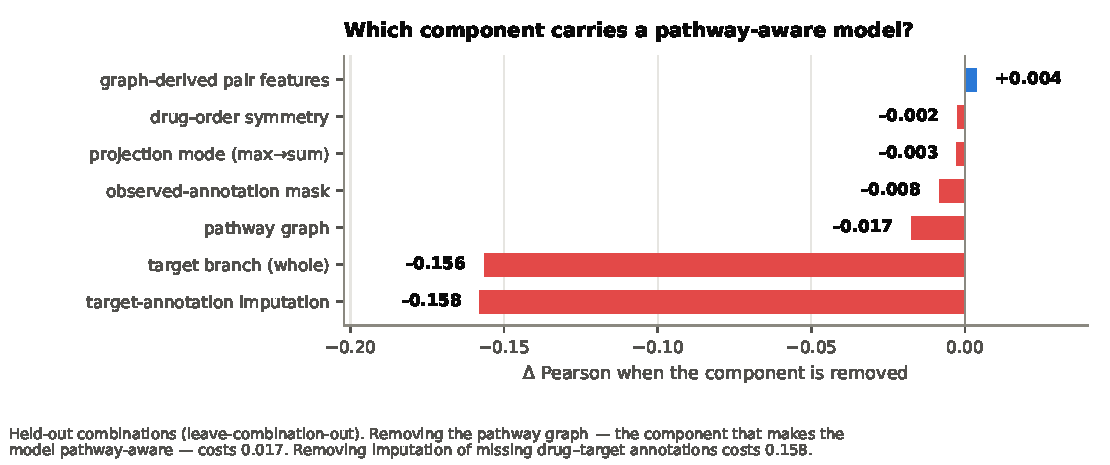
\includegraphics[width=0.7\textwidth]{fig2_ablation.pdf}}
\caption{Ablation deltas on {\tt leave\_combo\_out}. Only the pathway graph and
target-annotation imputation exceed the resolution floor, and they differ by an
order of magnitude.}
\label{fig:ablation}
\end{figure}

\begin{figure}[ht]
\centerline{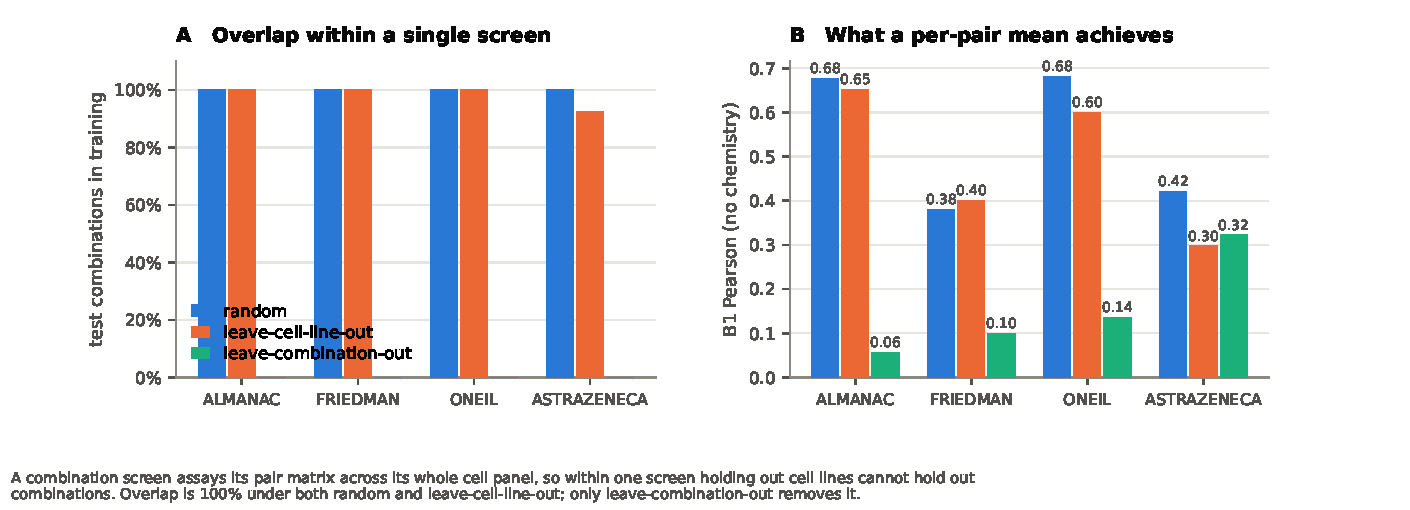
\includegraphics[width=\textwidth]{fig3_per_study.pdf}}
\caption{Per-study replication: within one screen the overlap is total. Each
contributing study assays its pair matrix across its whole cell panel, so every
held-out cell line still contains combinations seen in training.}
\label{fig:perstudy}
\end{figure}

\section{Discussion}

\paragraph{Recommendations.} Report combination overlap alongside any cold-start
result: no model, no retraining, no new data --- a property of the partition.
Where the claim concerns combination discovery, prefer {\tt leave\_combo\_out};
where it concerns external validity, prefer {\tt leave\_study\_out} (9.8\%
residual overlap). Report B1, or any context-plus-pair null model, as a routine
sanity check. Had it been reported, the leave-cell-line-out result would have
been visible immediately. These are concrete instances of the reporting practices
urged by REFORMS\cite{kapoor2024} and by Bernett et al.'s guiding
questions.\cite{bernett2024}

\paragraph{What this does not say.} Cold-cell-line prediction is not
uninteresting. Predicting how a known combination behaves in an uncharacterised
cell line is legitimate and clinically relevant --- it is simply not a test of
combination generalisation, and a model can excel at it while learning nothing
about chemistry. The two should not be conflated, and one number cannot serve
both.

\paragraph{Why this was not seen.} The protocols are named for what they hold
out, and the names are accurate: leave-cell-line-out does hold out cell lines.
The gap is between the entity held out and the entity the task concerns. Because
screens are dense in contexts and sparse in combinations, holding out the former
barely touches the latter. This is invisible from model performance alone; it
takes counting pairs.

\paragraph{Implications for structured biological priors.}
Sections~\ref{sec:verdict} and \ref{sec:ablation} together counsel caution in
attributing gains to biology. Where the pathway model helps, the effect is real
but small, and ablation locates most of its advantage in annotation completion.
Papers claiming benefits from biological priors would strengthen those claims by
ablating knowledge-injection and data-completion pathways separately.

\section{Limitations}\label{sec:limits}

\textbf{One corpus.} All results derive from DrugComb.
Section~\ref{sec:overlap} replicates the audit within four contributing screens,
addressing pooling but not the harmonisation.
\textbf{One instrument architecture.} Sections~\ref{sec:verdict} and
\ref{sec:ablation} rest on a single pathway model. We do not claim all such
models behave this way; we claim the attribution is unmeasured in work reporting
pathway benefits, and measuring it changes the interpretation.
\textbf{No published model re-evaluated.} We quantify overlap and demonstrate
consequences with our own baselines. Showing that specific published results
change under an overlap-controlled protocol requires re-running those methods,
and is the most important extension. The natural targets are
MatchMaker\cite{kuru2022} and the DrugCell subsystem model,\cite{kuenzi2020} the
latter being the canonical ``biological structure helps'' claim on which
Sec.~\ref{sec:ablation}'s attribution most directly bears.
\textbf{Baselines versus protocol.} Sec.~\ref{sec:invert} shows two non-neural
baselines beating two neural ones under high overlap; it does not by itself
establish that no neural model could recover the per-pair mean from embeddings. A
hybrid --- B3 given B1's per-cell and per-pair terms as features --- would
separate ``the protocol leaves too much signal'' from ``these particular networks
failed to learn an identifiable two-way effect'', and we regard it as the first
experiment a follow-up should run.
\textbf{Loewe regression only.} Reference models disagree
materially,\cite{vlot2019,duarte2022,fuentealba2023} so classification framings
and other metrics may behave differently. The overlap measurement is
metric-independent; the B1 consequences are not.
\textbf{Resolution floor.} Unpaired differences below about 0.007 Pearson are not
resolved (Sec.~\ref{sec:stats}); four ablation rows fall below it and are
reported as such.

\section{Conclusion}

Cold-start protocols in drug-combination synergy prediction hold out the entity
they name, but not always the entity the task concerns. Leave-cell-line-out and
leave-tissue-out retain most test combinations in training --- all of them within
a single screen --- and on that protocol a predictor with no molecular
information significantly outperforms neural models. Because the protocol
determines whether biological structure appears to help, be irrelevant, or hurt,
we recommend combination overlap and a context-plus-pair null model be reported
as standard. Both are essentially free, and both would have surfaced this.

\section*{Data and Code Availability}

Splits are persisted as row indices with a corpus fingerprint, reproducible
without redistributing the corpus. Ontology specifications carry a content hash
embedded in every checkpoint. The audit and null model run without a GPU in
minutes. Code and split definitions will be made publicly available upon
publication.

\section*{Use of Large Language Models}

A large language model was used as a coding and drafting assistant: for parts of
the analysis and plotting code, for LaTeX preparation, and for copy-editing of
author-written text. All experiments, numerical results, and scientific claims
were produced and verified by the authors, who take full responsibility for the
content.

\section*{Acknowledgments}

[TODO: funding sources and acknowledgments]

\bibliographystyle{ws-procs11x85}
\begin{thebibliography}{40}

\bibitem{preuer2018}
K.~Preuer, R.~P.~I. Lewis, S.~Hochreiter, A.~Bender, K.~C. Bulusu and
  G.~Klambauer, DeepSynergy: predicting anti-cancer drug synergy with Deep
  Learning, {\it Bioinformatics} {\bf 34}, 1538 (2018).

\bibitem{abbasi2024}
F.~Abbasi and J.~Rousu, New methods for drug synergy prediction: a mini-review,
  {\it Curr. Opin. Struct. Biol.}  (2024).

\bibitem{pan2023}
Y.~Pan {\it et~al.}, Review of Predicting Synergistic Drug Combinations, {\it
  Life}  (2023).

\bibitem{oneil2016}
J.~O'Neil, Y.~Benita, I.~Feldman, M.~Chenard, B.~Roberts, Y.~Liu {\it et~al.},
  An Unbiased Oncology Compound Screen to Identify Novel Combination Strategies,
  {\it Mol. Cancer Ther.} {\bf 15}, 1155 (2016).

\bibitem{holbeck2017}
S.~L. Holbeck, R.~Camalier, J.~A. Crowell, J.~P. Govindharajulu,
  M.~Hollingshead, L.~W. Anderson {\it et~al.}, The National Cancer Institute
  ALMANAC: A Comprehensive Screening Resource for the Detection of Anticancer
  Drug Pairs with Enhanced Therapeutic Activity, {\it Cancer Res.} {\bf 77}, 3564
  (2017).

\bibitem{zagidullin2019}
B.~Zagidullin, J.~Aldahdooh, S.~Zheng, W.~Wang, Y.~Wang, J.~Saad {\it et~al.},
  DrugComb: an integrative cancer drug combination data portal, {\it Nucleic
  Acids Res.} {\bf 47}, W43 (2019).

\bibitem{zheng2021}
S.~Zheng, J.~Aldahdooh, T.~Shadbahr, Y.~Wang, D.~Aldahdooh, J.~Bao {\it
  et~al.}, DrugComb update: a more comprehensive drug sensitivity data
  repository and analysis portal, {\it Nucleic Acids Res.} {\bf 49}, W174 (2021).

\bibitem{dewulf2021}
P.~Dewulf, M.~Stock and B.~De~Baets, Cold-Start Problems in Data-Driven
  Prediction of Drug-Drug Interaction Effects, {\it Pharmaceuticals} {\bf 14},
  p.~429 (2021).

\bibitem{monem2024}
S.~Monem {\it et~al.}, A multi-view feature representation for predicting drugs
  combination synergy based on ensemble and multi-task attention models, {\it J.
  Cheminform.}  (2024).

\bibitem{boonyarit2025}
B.~Boonyarit {\it et~al.}, SynProtX: a large-scale proteomics-based deep
  learning model for predicting synergistic anticancer drug combinations, {\it
  GigaScience}  (2025).

\bibitem{alam2024}
W.~Alam {\it et~al.}, Unlocking the therapeutic potential of drug combinations
  through synergy prediction using graph transformer networks, {\it Comput.
  Biol. Med.}  (2024).

\bibitem{kapoor2023}
S.~Kapoor and A.~Narayanan, Leakage and the reproducibility crisis in
  machine-learning-based science, {\it Patterns} {\bf 4}, p.~100804 (2023).

\bibitem{kapoor2022}
S.~Kapoor and A.~Narayanan, Leakage and the Reproducibility Crisis in ML-based
  Science, {\it arXiv}  (2022).

\bibitem{bernett2024}
J.~Bernett {\it et~al.}, Guiding questions to avoid data leakage in biological
  machine learning applications, {\it Nat. Methods}  (2024).

\bibitem{rosenblatt2024}
M.~Rosenblatt {\it et~al.}, Data leakage inflates prediction performance in
  connectome-based machine learning models, {\it Nat. Commun.}  (2024).

\bibitem{vlot2019}
A.~H.~C. Vlot, N.~Aniceto, M.~P. Menden, G.~Ulrich-Merzenich and A.~Bender,
  Applying drug synergy metrics to oncology combination screening data:
  agreements, disagreements and pitfalls, {\it Drug Discov. Today}  (2019).

\bibitem{duarte2022}
D.~Duarte and N.~Vale, Evaluation of synergism in drug combinations and
  reference models for future orientations in oncology, {\it Curr. Res.
  Pharmacol. Drug Discov.}  (2022).

\bibitem{roell2017}
K.~R. Roell, D.~M. Reif and A.~A. Motsinger-Reif, An Introduction to
  Terminology and Methodology of Chemical Synergy --- Perspectives from Across
  Disciplines, {\it Front. Pharmacol.}  (2017).

\bibitem{fuentealba2023}
O.~Fuentealba-Manosalva {\it et~al.}, Mind the Curve: Dose-Response Fitting
  Biases the Synergy Scores across Software Used for Chemotherapy Combination
  Studies, {\it Int. J. Mol. Sci.}  (2023).

\bibitem{ianevski2022}
A.~Ianevski, A.~K. Giri and T.~Aittokallio, SynergyFinder 3.0: an interactive
  analysis and consensus interpretation of multi-drug synergies across multiple
  samples, {\it Nucleic Acids Res.} {\bf 50}, W739 (2022).

\bibitem{yousefabadi2025}
H.~Yousefabadi {\it et~al.}, Bioactivity-Driven Prediction of Antibacterial
  Synergy Using Machine Learning Models, {\it bioRxiv}  (2025).

\bibitem{agboola2026}
O.~E. Agboola {\it et~al.}, End-to-end multimodal attention fusion for
  drug-target interaction prediction with cold-scaffold validation on the Davis
  kinase benchmark, {\it J. Mol. Graph. Model.}  (2026).

\bibitem{cheng2019}
F.~Cheng, I.~A. Kovacs and A.~L. Barabasi, Network-based prediction of drug
  combinations, {\it Nat. Commun.} {\bf 10}, p.~1197 (2019).

\bibitem{trac2025}
Q.~T. Trac {\it et~al.}, Pathway activation model for personalized prediction of
  drug synergy, {\it eLife}  (2025).

\bibitem{kuenzi2020}
B.~M. Kuenzi {\it et~al.}, Predicting Drug Response and Synergy Using a Deep
  Learning Model of Human Cancer Cells, {\it Cancer Cell} {\bf 38}, 672 (2020).

\bibitem{kuru2022}
H.~I. Kuru, O.~Tastan and A.~E. Cicek, MatchMaker: A Deep Learning Framework for
  Drug Synergy Prediction, {\it IEEE/ACM Trans. Comput. Biol. Bioinform.} {\bf
  19}, 2334 (2022).

\bibitem{sherine2025}
W.~B. Sherine {\it et~al.}, Graph Enhanced Transformers for Predicting Drug
  using Drug Synergies and Antagonistic Interactions, {\it ICESC}  (2025).

\bibitem{chen2023}
D.~Chen {\it et~al.}, Predicting anticancer synergistic drug combinations based
  on multi-task learning, {\it BMC Bioinformatics}  (2023).

\bibitem{wang2023}
Z.~Wang {\it et~al.}, DEML: Drug Synergy and Interaction Prediction Using
  Ensemble-Based Multi-Task Learning, {\it Molecules}  (2023).

\bibitem{preto2022}
A.~J. Preto {\it et~al.}, SYNPRED: prediction of drug combination effects in
  cancer using different synergy metrics and ensemble learning, {\it
  GigaScience}  (2022).

\bibitem{lin2023}
J.~Lin {\it et~al.}, Pisces: A multi-modal data augmentation approach for drug
  combination synergy prediction, {\it Cell Genomics}  (2023).

\bibitem{kapoor2024}
S.~Kapoor {\it et~al.}, REFORMS: Consensus-based Recommendations for
  Machine-learning-based Science, {\it Sci. Adv.}  (2024).

\bibitem{zhu2023}
J.~Zhu {\it et~al.}, Machine Learning in Environmental Research: Common Pitfalls
  and Best Practices, {\it Environ. Sci. Technol.}  (2023).

\bibitem{semmelrock2024}
H.~Semmelrock {\it et~al.}, Reproducibility in Machine Learning-based Research:
  Overview, Barriers and Drivers, {\it AI Magazine}  (2024).

\bibitem{liberzon2015}
A.~Liberzon, C.~Birger, H.~Thorvaldsdottir, M.~Ghandi, J.~P. Mesirov and
  P.~Tamayo, The Molecular Signatures Database (MSigDB) hallmark gene set
  collection, {\it Cell Syst.} {\bf 1}, 417 (2015).

\bibitem{szklarczyk2023}
D.~Szklarczyk, R.~Kirsch, M.~Koutrouli, K.~Nastou, F.~Mehryary, R.~Hachilif {\it
  et~al.}, The STRING database in 2023: protein-protein association networks and
  functional enrichment analyses for any sequenced genome of interest, {\it
  Nucleic Acids Res.} {\bf 51}, D638 (2023).

\bibitem{schubert2018}
M.~Schubert, B.~Klinger, M.~Klunemann, A.~Sieber, F.~Uhlitz, S.~Sauer {\it
  et~al.}, Perturbation-response genes reveal signaling footprints in cancer
  gene expression, {\it Nat. Commun.} {\bf 9}, p.~20 (2018).

\bibitem{tsherniak2017}
A.~Tsherniak, F.~Vazquez, P.~G. Montgomery, B.~A. Weir, G.~Kryukov, G.~S. Cowley
  {\it et~al.}, Defining a Cancer Dependency Map, {\it Cell} {\bf 170}, 564
  (2017).

\bibitem{ross2022}
J.~Ross, B.~Belgodere, V.~Chenthamarakshan, I.~Padhi, Y.~Mroueh and P.~Das,
  Large-scale chemical language representations capture molecular structure and
  properties, {\it Nat. Mach. Intell.} {\bf 4}, 1256 (2022).

\bibitem{zdrazil2024}
B.~Zdrazil, E.~Felix, F.~Hunter, E.~J. Manners, J.~Blackshaw, S.~Corbett {\it
  et~al.}, The ChEMBL Database in 2023: a drug discovery platform spanning
  multiple bioactivity data types and time periods, {\it Nucleic Acids Res.}
  {\bf 52}, D1180 (2024).

\end{thebibliography}

\end{document}
